\chapter{Results and discussion}
\label{chap:results}

\section{Characteristics of q\textsubscript{1} - q\textsubscript{2} stability diagrams for one electron}

%\subsection{Comparison of simulation and determinant stability criterion}

We will start by looking at the stability diagrams for different $\nicefrac{\Omega_2}{\Omega_1}$ ratios. Starting with \ref{fig:stabil-eta=3}.

\begin{figure}[H]
\begin{subfigure}{.5\textwidth}
  \centering
  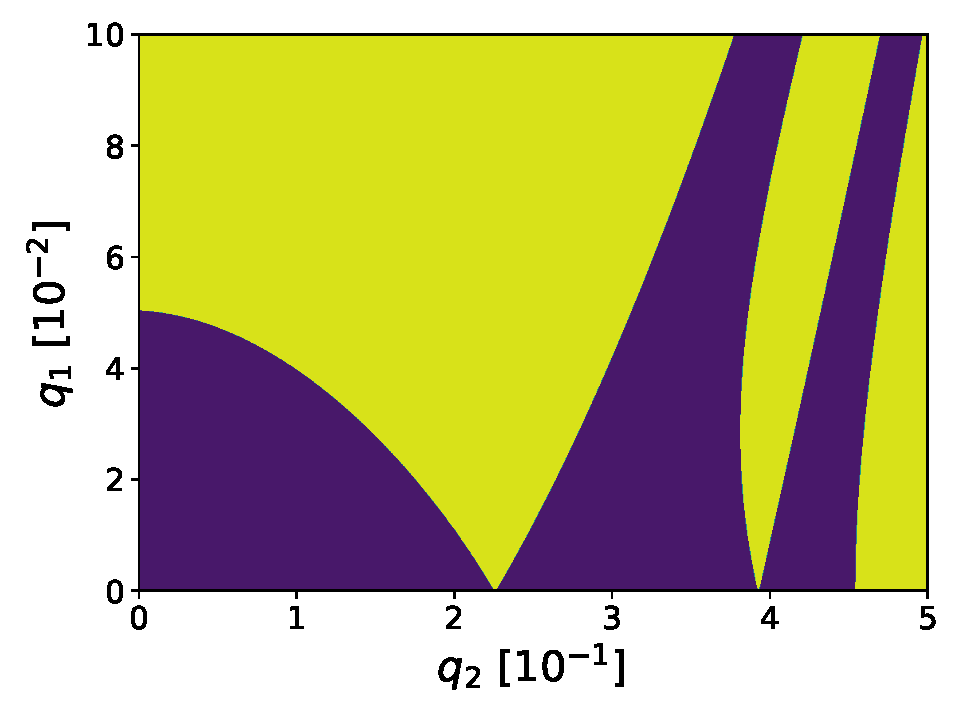
\includegraphics[width=\linewidth]{img/det_q1_0.0-0.1_q2_0.0-0.5_990x990_3.pdf}
  \caption{Determinant}
  \label{fig:det_3}
\end{subfigure}%
\begin{subfigure}{.5\textwidth}
  \centering
  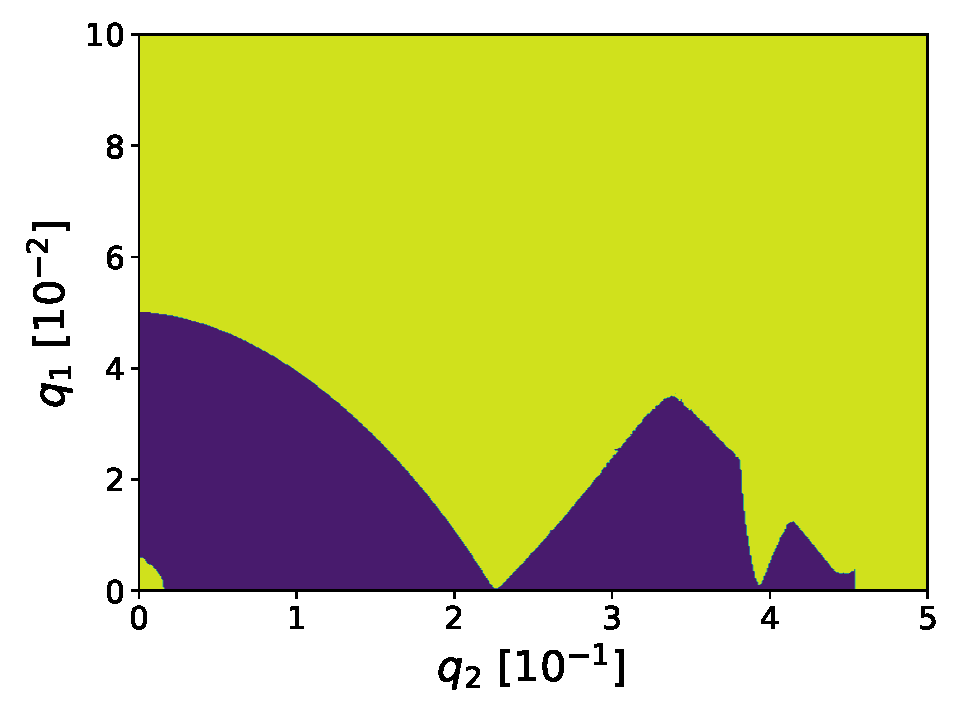
\includegraphics[width=\linewidth]{img/0_ions_1_electrons_q1_0.0-0.1_q2_0.0-0.5_488x488_3.pdf}  
  \caption{Simulation}
  \label{fig:sim_3}
\end{subfigure}
\caption{Stability diagrams for $\nicefrac{\Omega_2}{\Omega_1} = 3$}
\label{fig:stabil-eta=3}
\end{figure}

In the figure \ref{fig:stabil-eta=3} we can see regions of stable\textit{(dark)} and unstable\textit{(light)} solutions to our equation of motion. The picture \ref{fig:det_3} was determined with use of Floquet theory. The adjacent image shows the stability of an electron based on numerical simulation. In contrast with the determinant solution, we can see some evident distinctions. The around $q_1 \approx q_2 \approx 0$ became unstable. This is no surprise since such a weak field did not satisfy the requirement \eqref{stability condition inequality} for the given initial conditions. More importantly, two whole stability areas have melted away in the field with higher amplitudes. We must not forget that the stability in the figure \ref{fig:det_3} is calculated only along the z-axis. We can investigate this by setting the initial position and velocity in x-y directions to zero. As we can see, the subsequent picture \ref{fig:sim_3_z-direction} already agrees with the determinant solution \ref{fig:det_3}.

\begin{figure}[H]
\begin{subfigure}{.5\textwidth}
  \centering
  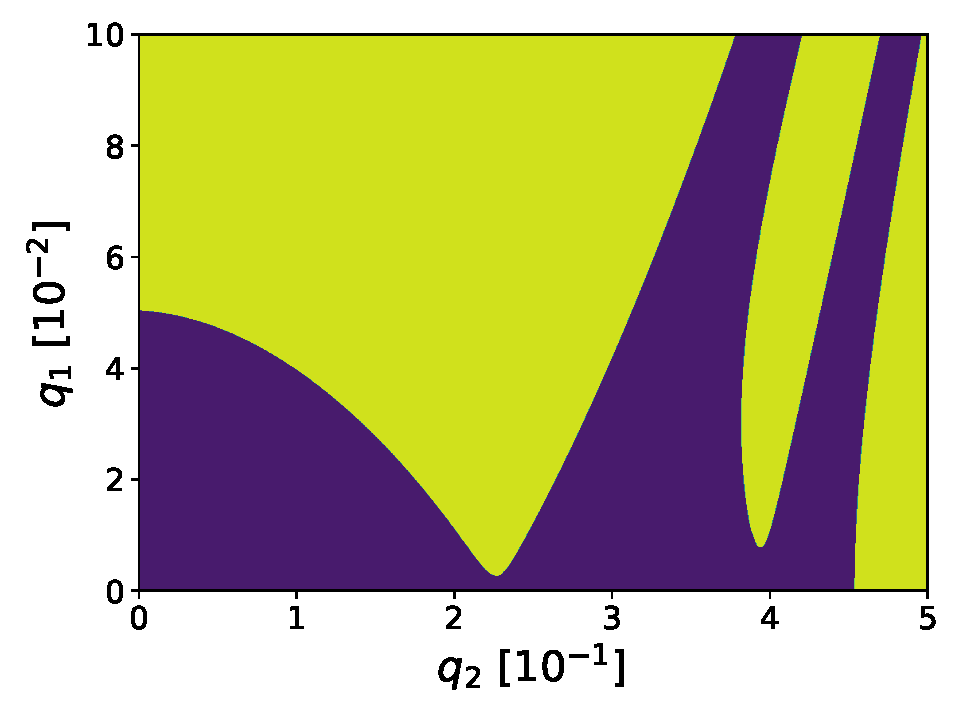
\includegraphics[width=\linewidth]{img/0_ions_1_electrons_q1_0.0-0.1_q2_0.0-0.5_992x992_3.pdf}
  \caption{Simulation in z-direction}
  \label{fig:sim_3_z-direction}
\end{subfigure}%
\begin{subfigure}{.5\textwidth}
  \centering
  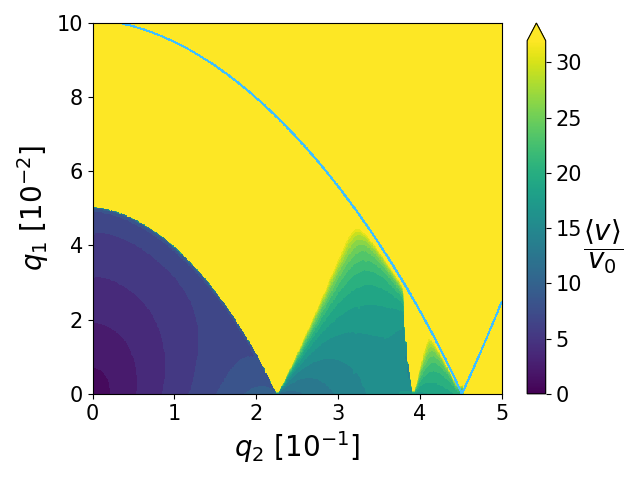
\includegraphics[width=\linewidth]{img/det_q1_0.0-0.1_q2_0.0-0.5_970x970_3_1000.png}  
  \caption{Average velocity simulated in 3D}
  \label{fig:sim_3_x-y_edge}
\end{subfigure}
\caption{Stability diagrams for $\nicefrac{\Omega_2}{\Omega_1} = 3$}
\label{fig:stabil-eta=3 different directions}
\end{figure}

In the next set of pictures \ref{fig:stabil-eta=3_x-y_directions}, we evaluate the stability diagram in x-y directions by setting $\zeta = x$ in \eqref{tilde params} for a determinant solution and setting the z-component of initial position and velocity to zero in the simulation. The red trace in both pictures embodies the edge of stability made with our standard \eqref{stability condition in simulation} stability requirement in simulation. The contour plot in \ref{fig:sim_3_x-direction} was created with the enhanced condition for identifying stable solutions from the standard \eqref{stability condition in simulation} to $\max\limits_{x \in \mathcal{L}}(r) \leq 2 \ \ell_0$, while increasing the total simulation time as well. So this picture \ref{fig:sim_3_x-direction}, among other things, illustrates the non-equivalence of our stability condition while simulating and the condition of stability we use in Floquet theory, as we have already mentioned in \ref{foot:different stability condition}. 

In the background of \ref{fig:sim_3_x-y_edge} is a contour plot of the average electron velocity $\langle v \rangle$ throughout the whole trajectory\footnote{Average value defined as: $\langle \xi \rangle = \nicefrac{1}{T} \int_{0}^{T} \xi(\tau) \, d\tau,$ where $T$ denotes a total time of simulation.} relative to the initial velocity $v_0$. The color bar to the right indicates the value of this ratio. We create all the other figures similar to \ref{fig:sim_3_x-y_edge} in the same way. These diagrams can help us find stable trap parameters while keeping electron temperature as low as possible, which is our ultimate goal. The light blue line in \ref{fig:sim_3_x-y_edge} represents the stability edge taken from \ref{fig:stabil-eta=3_x-y_directions}, delivering a crucial message about the difference between the two stability diagrams in \ref{fig:stabil-eta=3}. We see that our discrepancy problem between determinant and simulated stability diagrams is settled by the obvious necessity to combine determinant solutions in both x and z directions. This can be easily fixed with the cost of doubling the computation time for a determinant solution. Nonetheless, from now on, we will focus on simulated results, keeping the determinant diagrams in the z-direction for comparison. Moreover, we can use these pictures \ref{fig:stabil-eta=3_x-y_directions} as a sanity check. By matching them with the results from \cite{leefer2017investigation} \textit{(where the stability of the ideal quadrupole trap along the x-direction was studied)}, we see that we have reproduced the same\footnote{Note that we are using different condition to identify stable solutions.} results $\rightarrow$ proving the validity of our code, at least to some extent.
\begin{figure}[H]
\begin{subfigure}{.5\textwidth}
  \centering
  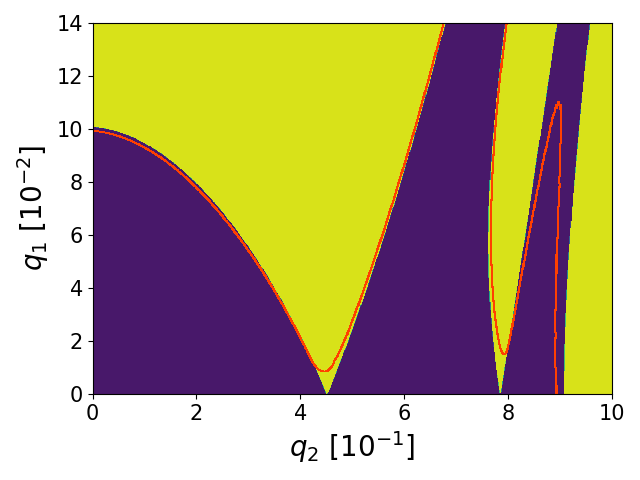
\includegraphics[width=\linewidth]{img/0_ions_1_electrons_q1_0.0-0.14_q2_0.0-1.0_992x984_3_edge.png}%det_q1_0.0-0.14_q2_0.0-1.0_960x960_3.pdf not sure which one to use
  \caption{Determinant in x-direction}
  \label{fig:det_3_x-direction}
\end{subfigure}%
\begin{subfigure}{.5\textwidth}
  \centering
  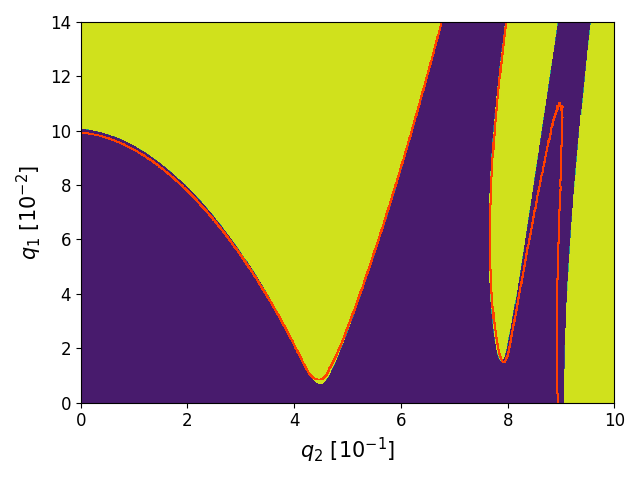
\includegraphics[width=\linewidth]{img/0_ions_1_electrons_q1_0.0-0.14_q2_0.0-1.0_992x984_3_edge_sim.png}  
  \caption{Simulation in x-y plane}
  \label{fig:sim_3_x-direction}
\end{subfigure}
\caption{Stability diagrams for $\nicefrac{\Omega_2}{\Omega_1} = 3$ in x-y plane}
\label{fig:stabil-eta=3_x-y_directions}
\end{figure} 
The image \ref{fig:velocityedge-eta=3} again combines two pictures. The pink curve from now on construes the stable simulated regions, in this case, taken for \ref{fig:sim_3}. 
\begin{figure}[H]
	\centering
	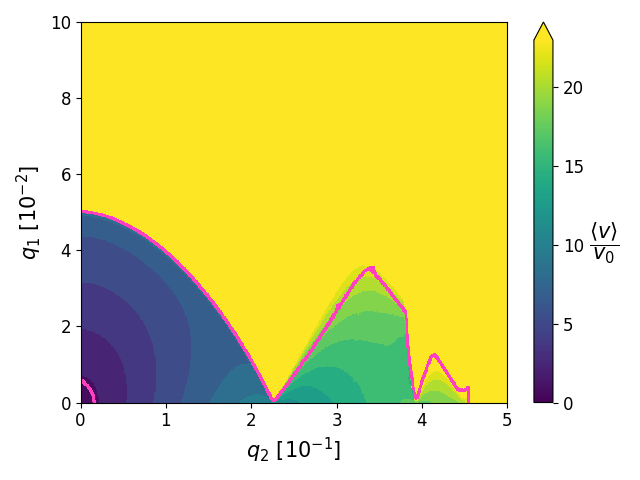
\includegraphics[width=\linewidth]{img/0_ions_1_electrons_q1_0.0-0.1_q2_0.0-0.5_488x488_3_1000.png}
	\caption{Average electron velocity for $\nicefrac{\Omega_2}{\Omega_1} = 3$}
	\label{fig:velocityedge-eta=3}
\end{figure}

Moving to larger frequency ratio $\rightarrow \nicefrac{\Omega_2}{\Omega_1} = 13$ we can start to notice some patterns.

\begin{figure}[H]
\begin{subfigure}{.5\textwidth}
  \centering
  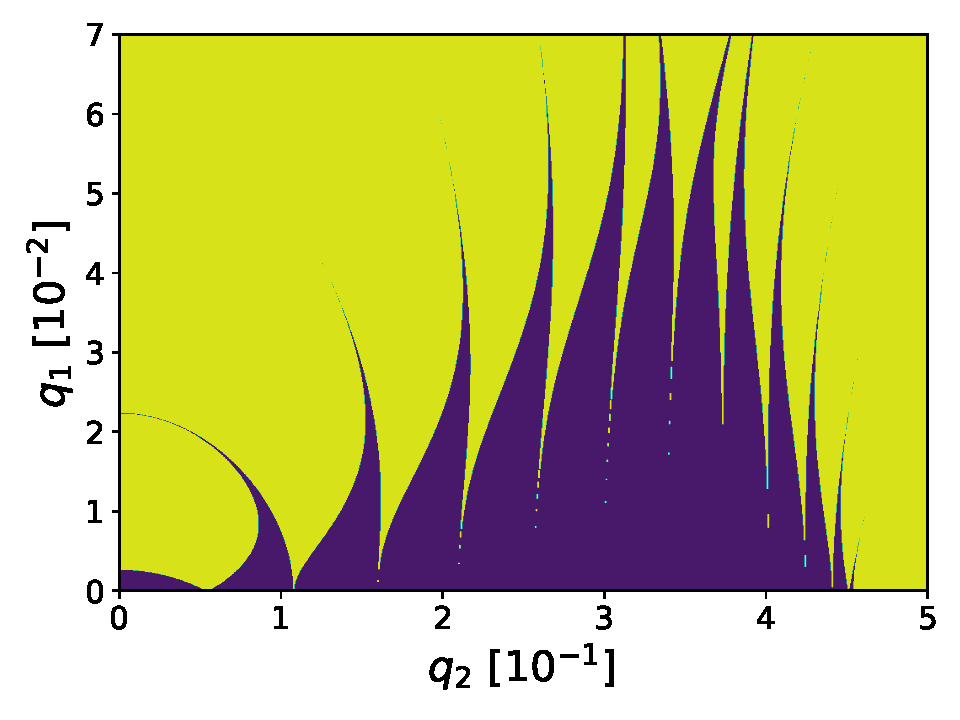
\includegraphics[width=\linewidth]{img/det_q1_0.0-0.07_q2_0.0-0.5_960x960_13.pdf}
  \caption{Determinant}
  \label{fig:det_13}
\end{subfigure}%
\begin{subfigure}{.5\textwidth}
  \centering
  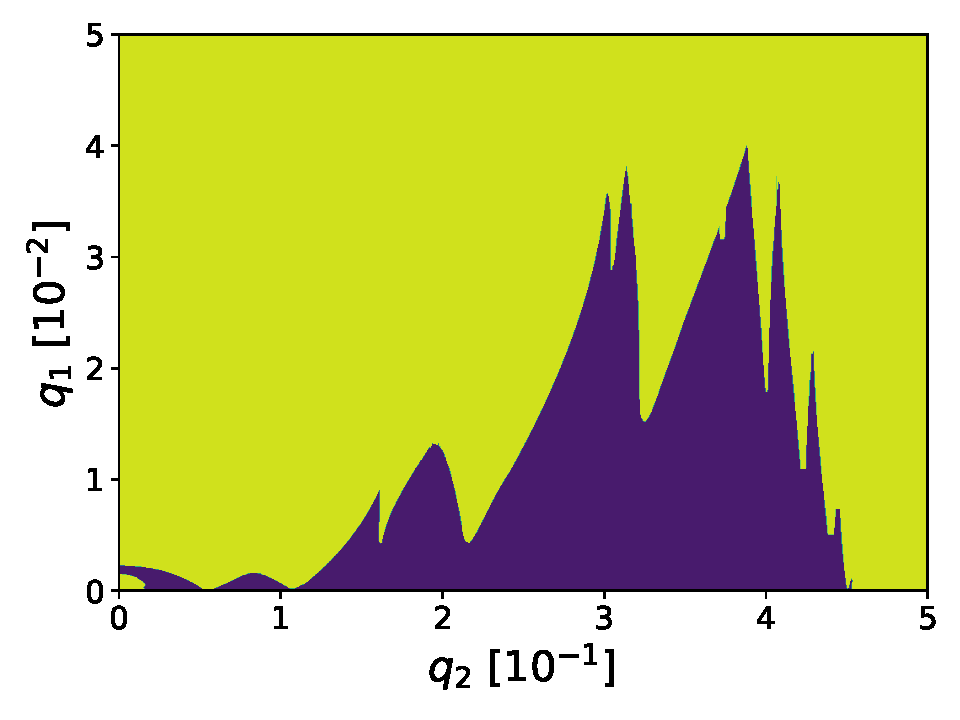
\includegraphics[width=\linewidth]{img/0_ions_1_electrons_q1_0.0-0.05_q2_0.0-0.5_960x960_13.pdf}  
  \caption{Simulation}
  \label{fig:sim_13}
\end{subfigure}
\caption{Stability diagrams for $\nicefrac{\Omega_2}{\Omega_1} = 13$}
\label{fig:velocityedge-eta=13}
\end{figure}

\begin{figure}[H]
	\centering
	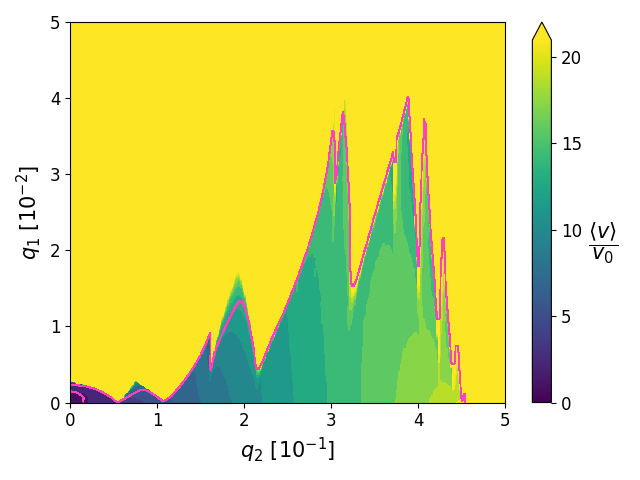
\includegraphics[width=\linewidth]{img/0_ions_1_electrons_q1_0.0-0.05_q2_0.0-0.5_960x960_13_1000.png}
	\caption{Average electron velocity for $\nicefrac{\Omega_2}{\Omega_1} = 13$}
	\label{fig:stabil-eta=13}
\end{figure}

There emerges one stable triangle with many tongues of instability. With an increasing ratio $\nicefrac{\Omega_2}{\Omega_1}$ we can see a gain in the number of these tongues, but their width promptly shrinks as well. We expect that by further increasing the frequency ratio, the unstable tongues will be realistically affecting only the regions near the edge of stability, leaving the regions further inside a stable triangle safe to work with.

Continuing to the frequency ratio compatible for trapping electrons and Ca+ ions $\rightarrow \nicefrac{\Omega_2}{\Omega_1} = 833$

\begin{figure}[H]
\begin{subfigure}{.5\textwidth}
  \centering
  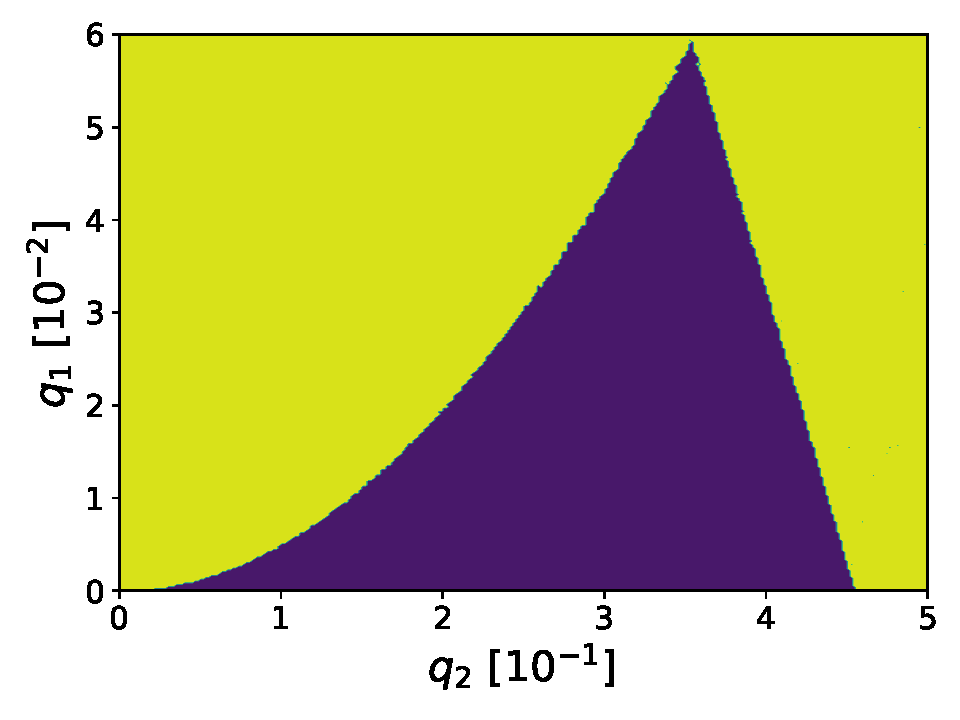
\includegraphics[width=\linewidth]{img/det_q1_0.0-0.06_q2_0.0-0.5_300x300_833.pdf}
  \caption{Determinant}
  \label{fig:det_833}
\end{subfigure}%
\begin{subfigure}{.5\textwidth}
  \centering
  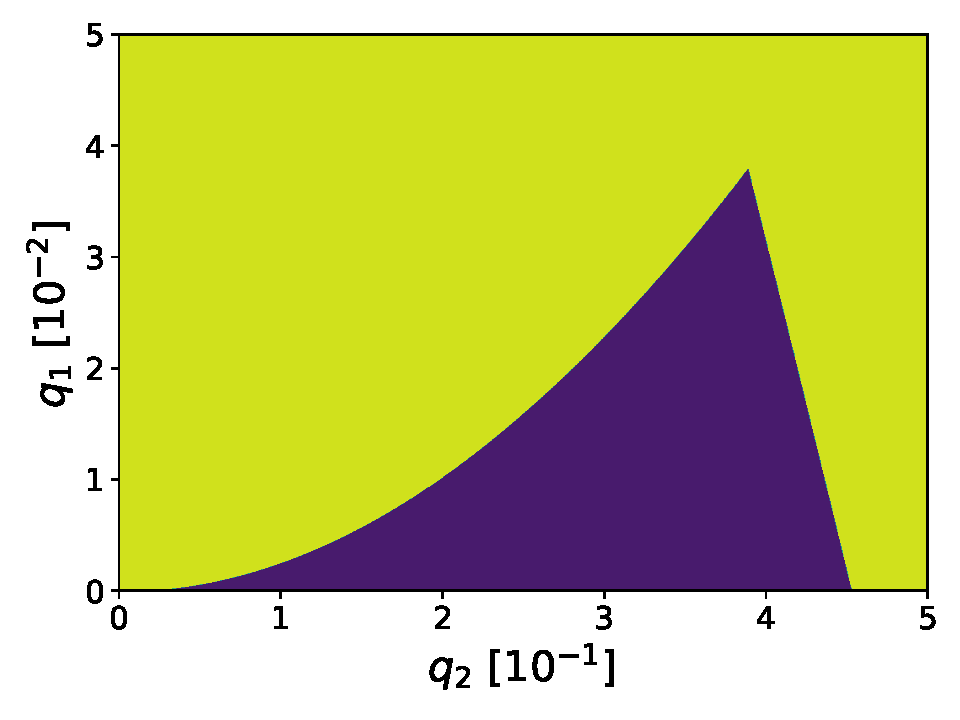
\includegraphics[width=\linewidth]{img/0_ions_1_electrons_q1_0.0-0.05_q2_0.0-0.5_960x960_833.pdf}  
  \caption{Simulation}
  \label{fig:sim_833}
\end{subfigure}
\caption{Stability diagrams for $\nicefrac{\Omega_2}{\Omega_1} = 833$}
\label{fig:stabil-eta=833}
\end{figure}

At this point, the unstable tongues became so dense and narrow that we practically could not see them in stability diagrams \ref{fig:stabil-eta=833}. The closeup was evaluated after a thousand secular oscillations, and the tongues vanished virtually instantly. The stability triangle will continue to shrink with an increasing frequency ratio. However, the character of this region will stay the same. Therefore, predicting stability for different frequency ratios in this range is simple. The essential information comes from the figure \ref{fig:vel-eta=833}. As we can see, an electron's average velocity drops in weaker fields, furnishing us with a method to reach lower electron velocities. Imagine we have already set up a CC in a field that is also stable for electrons. Assuming the electron can cool itself by interactions with Rydberg ions, we follow by gradual change of trapping parameters aiming towards the weak field region. Such will be simulated in the future.

It is worth pointing out that the computation time of the determinant stability diagram already exceeds that of simulated for a frequency ratio this big. However, we apply a built-in NumPy\footnote{NumPy is widely used, open source, numerical python library: \href{https://numpy.org}{https://numpy.org/}} function for computing determinants using LU decomposition \cite{teukolsky1992numerical} with time complexity $\mathcal{O}(n^3)$, not utilizing the fact that our matrices are sparse. Moreover, we are interested only in the sign of a determinant which also suggests a capacity for efficiency improvement. But since the determinant solutions are not essential to us, we do not investigate such further advancements in this thesis.

\begin{figure}[H]
	\centering
	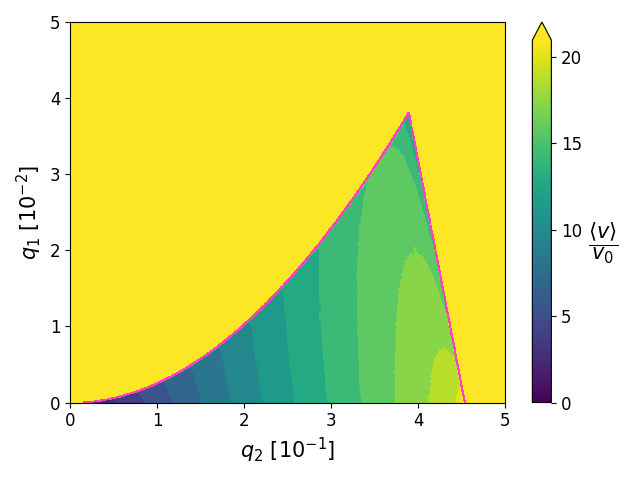
\includegraphics[width=\linewidth]{img/0_ions_1_electrons_q1_0.0-0.05_q2_0.0-0.5_960x960_833_1000.png}
	\caption{Average electron velocity for $\nicefrac{\Omega_2}{\Omega_1} = 833$}
	\label{fig:vel-eta=833}
\end{figure}

\begin{figure}[H]
\begin{subfigure}{.5\textwidth}
  \centering
  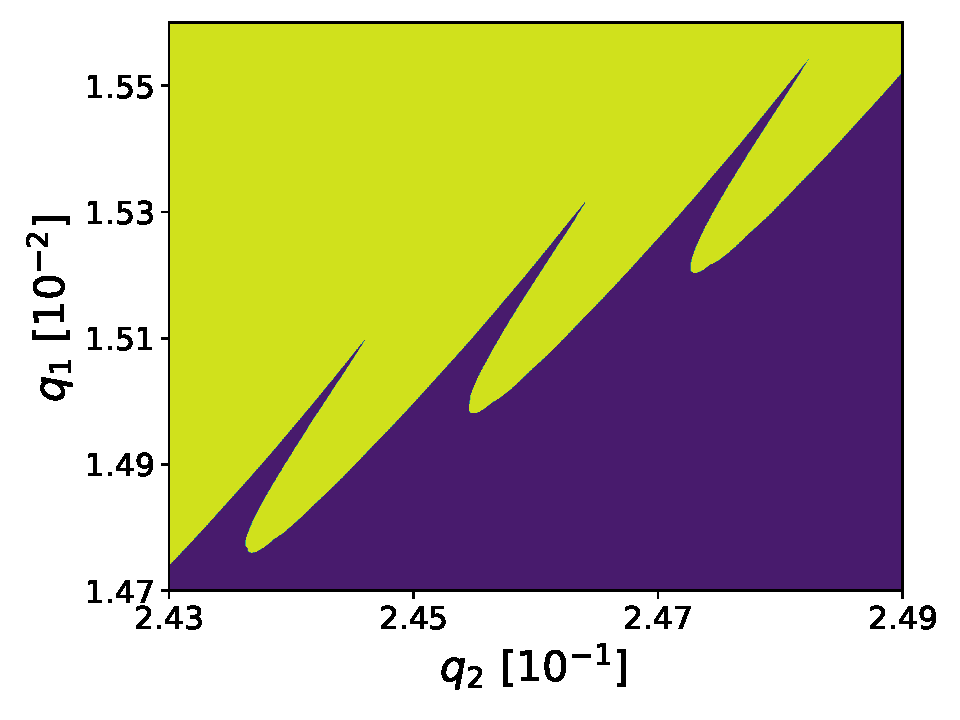
\includegraphics[width=\linewidth]{img/0_ions_1_electrons_q1_0.0147-0.0156_q2_0.243-0.249_960x960_833.pdf}
  %\caption{Determinant}
  \label{fig:sim-edge_833}
\end{subfigure}%
\begin{subfigure}{.5\textwidth}
  \centering
  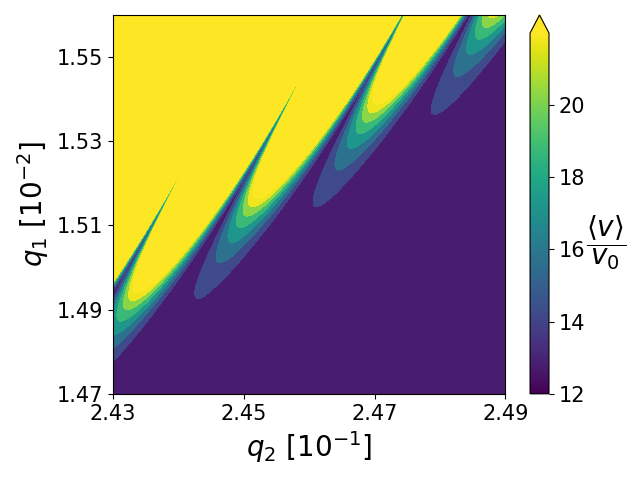
\includegraphics[width=\linewidth]{img/0_ions_1_electrons_q1_0.0147-0.0156_q2_0.243-0.249_220x220_833.png}  
  %\caption{Simulation}
  \label{fig:sim-edge-vel_833}
\end{subfigure}
\caption{Simulated edge of stability for $\nicefrac{\Omega_2}{\Omega_1} = 833$}
\label{fig:stabil-edge-eta=833}
\end{figure}

\begin{figure}[H]
	\centering
	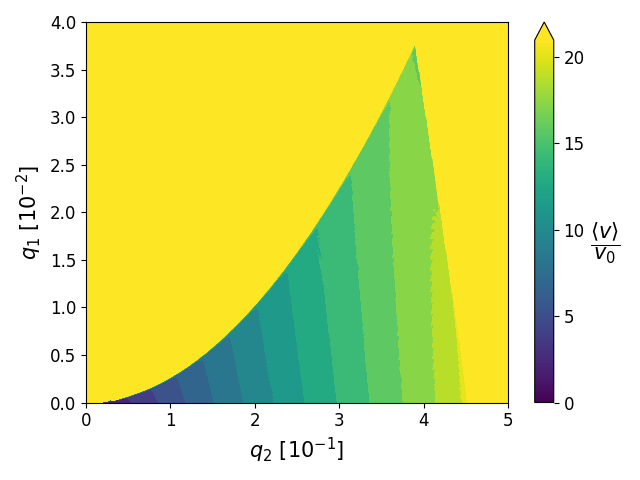
\includegraphics[width=\linewidth]{img/0_ions_1_electrons_q1_0.0-0.04_q2_0.0-0.5_360x360_1207.png}
	\caption{Average electron velocity for $\nicefrac{\Omega_2}{\Omega_1} = 1207$}
	\label{fig:vel-eta=1207}
\end{figure}

\section{Creating a Coulomb crystal}

As we have already mentioned, we assemble a CC by solving the equation of motion for each ion in an effective potential with damping and mutual Coulombic interaction. Such an equation has the form:\todo{finish this}

\begin{figure}[H]
\begin{subfigure}{.5\textwidth}
  \centering
  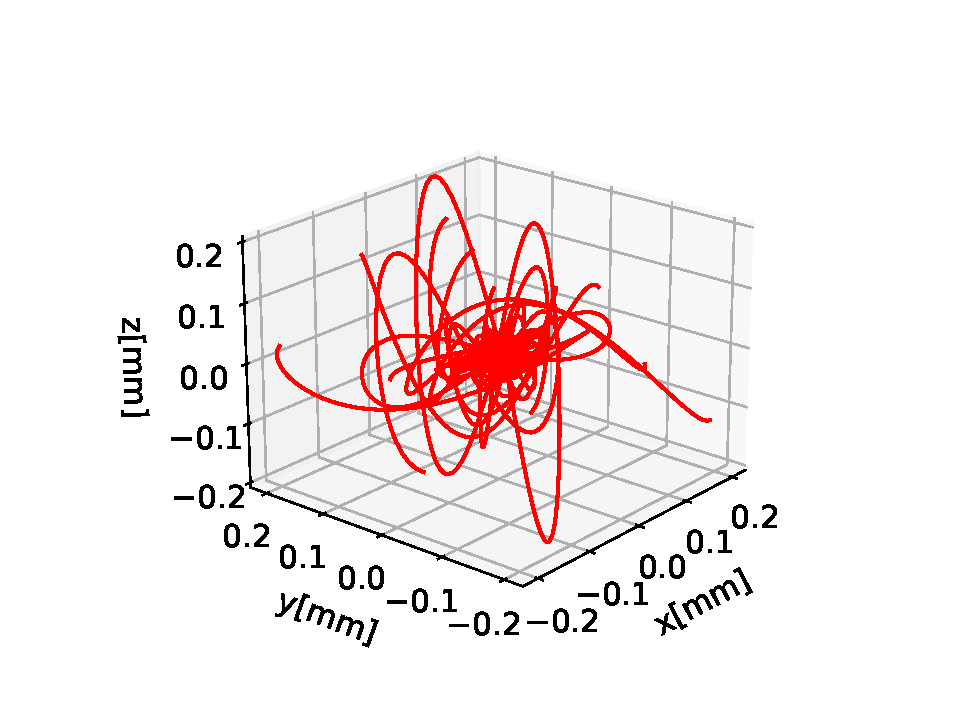
\includegraphics[width=\linewidth]{img/CC_10.pdf}
  \caption{Simulating multiple ions in effective potential with damping}
\end{subfigure}%
\begin{subfigure}{.5\textwidth}
  \centering
  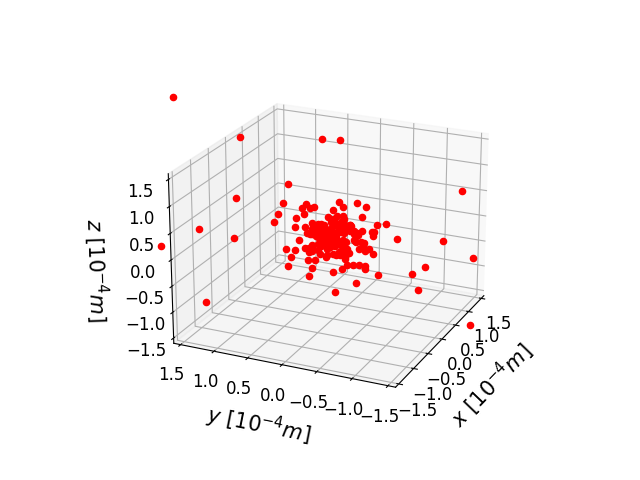
\includegraphics[width=\linewidth]{img/CC_200.png}  
  \caption{Assembling a CC (200 ions)}
\end{subfigure}
\caption{Creating CC $\nicefrac{\Omega_2}{\Omega_1} = 1207$}
\label{fig:CC-eta=1207}
\end{figure}

\section{Stability of electron in Coulomb crystal}

The ions stand practically still in the time scales corresponding to twenty secular electron oscillations. Therefore, while computing stability diagrams in the presence of CCs, we freeze ions in place, rapidly improving computational time.


\xxx{We have simulated motion of an electron inside ideal Paul trap in the presence of CC with up to 200 ions in it, but it had no impact on the electron's stability. Potential instabilities may arise only on longer time scales, which has to be investigated further.}
\todo{continue simulating with more ions\dots}
\section{Future}

Our concerns in the future will be reproducing results of this thesis for the real planar geometry of the trap used in our experiment. The potential of such a trap can be formulated in integral form utilizing Bessel functions, which will make our simulations much more computationally expensive. We need to derive equation of motion and identify parameters analogous to $a$, $q_1$ and $q_2$ which we had for ideal quadrupole trap. After that we can use our exiting program to study stability of particles in dependence on such parameters exactly as we did in this thesis. 